\documentclass{crypto-exercise}
\usepackage{pgfplots}

\author{Sven Laur}
\contributor[Initial draft]{Lembit Valgma}
\tags{random self-reducibility, time-success profile}


\begin{document}
\begin{exercise}{Random self-reducibility and time-success profile}
Many security assumptions can be viewed as inversion tasks. More precisely, there exists 
an efficiently computable function $f:\XXX\to\YYY$ such that a security assumption $\mathfrak{P}$ is satisfied 
when for any $t$-time algorithm $\AD$:
\begin{align*}
\ADV_{\XXX}^\mathfrak{P}(\AD)=\pr{x\getsu\XXX: \AD(f(x))=x}\leq\varepsilon\enspace.
\end{align*}
Study what implications does random self-reducibility add to the time success profile $\varepsilon(t)$.

\end{exercise}
\begin{solution}
Recall that time-success profile $\varepsilon(t)$  corresponds to the maximal success for each time bound, which can be further compressed into a single number by considering the best time-success ratio over the entire time-success profile:
\begin{align*}
\alpha = \min_t \frac{t}{\varepsilon(t)}\enspace.
\end{align*}
Intuitively, the time-success ratio shows the minimal time that is needed to  reverse the function with complete certainty, as a single run will succeed with probability $\varepsilon(t)$. Consequently, we need to repeat the procedure at least $\frac{1}{\varepsilon(t)}$-times to cover the entire probability space. The latter is only an estimate, since the second run of an algorithm does not have to succeed when the first run fails. If the problem is randomly self-reducible then the outcomes of individual runs are uncorrelated and we can formally justify the intuition. 

\vspace*{2ex}
\noindent
\textsc{Near-linear behaviour.}
Random self-reducibility in our context means that inverting any instance of $f(x)$ can be reduced to inversion of a random instance in $\YYY$. More formally, there exist efficiently computable re-randomisation function 
\begin{align*}
h: \YYY\times\RRR\to\YYY
\end{align*}
and its inverse for the solution recovery
\begin{align*}
g: \XXX\times\RRR\to\XXX
\end{align*}
such that following conditions are met. First, for any $f(x)\in\YYY$ the outcome $h(f(x), r)$ has uniform distribution over $\YYY$ whenever $r$ is chosen uniformly from $\RRR$. Second, a solution $x_*$ for the randomised instance $h(f(x),z)$ can be converted back to a solution for the original problem:
\begin{align}
\label{eq:random-selfreducibility}
\forall r\in\RRR:\,\forall x_*\in\XXX:\quad f(x_*) = h(f(x),r) 
\Longrightarrow
f(g(x_*,r))=f(x)\enspace.
\end{align}
If these functions exist, we can convert $t$-time adversary $\AD$ to an adversary with time complexity $\Theta(\ell t)$ 
\begin{align*}
\begin{fblock}{\ADB(y)}
 &\begin{forblock}{i \in\set{1,\ldots,\ell}}
 &r\gets\RRR\\
 &x_*\gets\AD(h(y, r)) \\
 &x\gets g(x_*,r)\\
 &\IF f(x)=y\ \THEN \RETURN x
 \end{forblock}\\
 &\RETURN \bot\enspace.
\end{fblock}
\end{align*} 
More precisely, the running time of $\ADB$ is $\ell(t_h+t+t_g+t_f)$ where $t_f,t_g,t_h$ are running times for evaluating functions $f, g, h$.  Equation~\eqref{eq:random-selfreducibility} guarantees that $\ADB$ succeeds whenever $\AD$ succeeds. The first property guarantees that each call to $\AD$ is an independent and random problem instance. Thus, the probability of a failure is 
\begin{align*}
\pr{\ADB(y)=\bot} = (1-\varepsilon)^\ell\enspace.
\end{align*}
The inequalities stemming from exclusion-inclusion principle assure that
\begin{align*}
1 -\ell\varepsilon\leq (1-\varepsilon)^\ell \leq 1 -\ell\varepsilon +\frac{\ell(\ell-1)}{2}\varepsilon^2 
\end{align*}
and thus we have bounds for the success probability:
\begin{align*}
\ell\varepsilon\left(1-\frac{\varepsilon(\ell-1)}{2}\right) \leq\pr{x\gets \ADB(y): f(x)=y}\leq \ell\varepsilon\enspace.
\end{align*}
Note that as long as $\ell \ll \frac{1}{\varepsilon}$ the lower bound is negligibly close to the upper bound and the success probability grows indeed  linearly for all practical purposes.

\vspace*{2ex}
\noindent
\textsc{Regime shift to exponential saturation.}
Let us now observe the behaviour when $\ell$ is around $\frac{1}{\varepsilon}$ and thus the approximation outlined above is imprecise. Bernoulli's inequality  implies that for any $\varepsilon\in (0,1]$
\begin{align*}
(1-\varepsilon)^{1/\varepsilon}\leq  \frac{1}{e} 
\end{align*}
and thus the success probability converges exponentially  fast to one:
\begin{align*}
\pr{x\gets \ADB(y): f(x)=y} = 1- (1-\varepsilon)^\ell\geq 1 - e^{-\varepsilon\ell}\enspace.
\end{align*}

\vspace*{2ex}
\noindent
\textsc{Connection to maximal time-success ratio.}
Let $\AD$ be $t$-time algorithm that achieves the best time-success ratio $\alpha$. Then we can construct $(\alpha+t)$-time algorithm by doing $\ell=\ceil{1/\varepsilon}$ repetitions. Consequently, the success of the algorithm is at least $1-1/\varepsilon\geq 0.63$ and thus the naive hope that there exist $\alpha$-time algorithm that completely solves the problem is not so far off.

\vspace*{2ex}
\noindent
\textsc{Generic square root algorithm.}
Note that by tabulating $\ell$ values of $f(x)$ we can succeed with probability $\frac{\ell}{\abs{\XXX}}$ for a random inversion instance. By doing $\ell$ trials we can amplify this probability to
\begin{align*}
\pr{x\gets \ADB(y): f(x)=y}\geq
\frac{\ell^2}{\abs{\XXX}}\cdot\left(1-\frac{\ell(\ell-1)}{2\abs{\XXX}}\right)\enspace,
\end{align*}
which is a near-quadratic function for $\ell\leq\sqrt{\abs{\XXX}}$. A naive implementation of this algorithm, which tabulates $f$ each time, also runs in quadratic time. However, if we cache the tabulation results, the running-time becomes linear in $\ell$ and thus we get a quadratic lower bound to time-success profile $\varepsilon(t)$.
 
\vspace*{2ex}
\noindent
\textsc{Restrictions to the time-success profile.}
The following figure shows sharpness and relations between bounds and fixes a region where the time-success profile must be located. \begin{center}
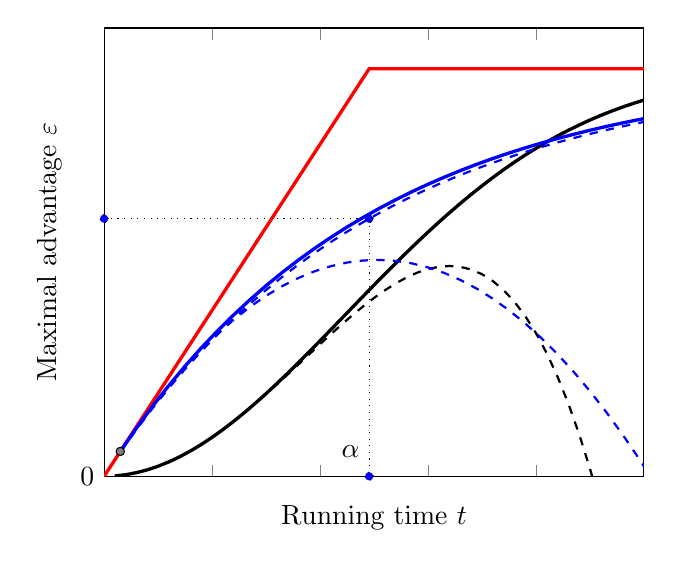
\begin{tikzpicture}
\begin{axis}[
    xlabel={Running time $t$ },
    ylabel={Maximal advantage $\varepsilon$},
    xmin=0, xmax=100,
    ymin=0, ymax=1.1,
    xtick={0,20,40,60,80,100},
    xticklabels={,,},
    ytick={0,20,40,60,80,100,120},
]
 
% Exact tabulation algorithm 
\addplot[color=black, very thick] coordinates 
{(2, 0.0010)(4, 0.0040)(6, 0.0090)(8, 0.0159)(10, 0.0248)(12, 0.0355)(14, 0.0480)(16, 0.0622)(18, 0.0781)(20, 0.0956)(22, 0.1146)(24, 0.1349)(26, 0.1564)(28, 0.1791)(30, 0.2028)(32, 0.2275)(34, 0.2528)(36, 0.2789)(38, 0.3054)(40, 0.3324)(42, 0.3596)(44, 0.3870)(46, 0.4144)(48, 0.4418)(50, 0.4690)(52, 0.4959)(54, 0.5224)(56, 0.5485)(58, 0.5741)(60, 0.5990)(62, 0.6233)(64, 0.6468)(66, 0.6696)(68, 0.6915)(70, 0.7126)(72, 0.7328)(74, 0.7522)(76, 0.7706)(78, 0.7881)(80, 0.8046)(82, 0.8203)(84, 0.8351)(86, 0.8489)(88, 0.8619)(90, 0.8741)(92, 0.8854)(94, 0.8959)(96, 0.9057)(98, 0.9147)(100, 0.9231)(102, 0.9307)(104, 0.9378)(106, 0.9442)(108, 0.9501)(110, 0.9555)(112, 0.9603)(114, 0.9647)(116, 0.9687)(118, 0.9723)(120, 0.9756)(122, 0.9785)(124, 0.9811)(126, 0.9834)(128, 0.9855)(130, 0.9873)(132, 0.9890)(134, 0.9904)(136, 0.9917)(138, 0.9928)(140, 0.9938)(142, 0.9946)(144, 0.9954)(146, 0.9960)(148, 0.9966)(150, 0.9971)(152, 0.9975)(154, 0.9979)(156, 0.9982)(158, 0.9985)(160, 0.9987)(162, 0.9989)(164, 0.9991)(166, 0.9992)(168, 0.9994)(170, 0.9995)(172, 0.9996)(174, 0.9996)(176, 0.9997)(178, 0.9998)(180, 0.9998)(182, 0.9998)(184, 0.9999)(186, 0.9999)(188, 0.9999)(190, 0.9999)(192, 0.9999)(194, 0.9999)(196, 1.0000)(198, 1.0000)(200, 1.0000)};

% Lower bound to tabulation algorithm     
\addplot[color=black, thick, dashed] coordinates 
{(2, 0.0010)(4, 0.0040)(6, 0.0090)(8, 0.0159)(10, 0.0248)(12, 0.0355)(14, 0.0480)(16, 0.0622)(18, 0.0781)(20, 0.0955)(22, 0.1143)(24, 0.1345)(26, 0.1558)(28, 0.1782)(30, 0.2014)(32, 0.2253)(34, 0.2497)(36, 0.2744)(38, 0.2993)(40, 0.3240)(42, 0.3484)(44, 0.3722)(46, 0.3952)(48, 0.4170)(50, 0.4375)(52, 0.4563)(54, 0.4731)(56, 0.4876)(58, 0.4996)(60, 0.5085)(62, 0.5141)(64, 0.5161)(66, 0.5140)(68, 0.5075)(70, 0.4961)(72, 0.4795)(74, 0.4572)(76, 0.4289)(78, 0.3939)(80, 0.3520)(82, 0.3026)(84, 0.2452)(86, 0.1794)(88, 0.1045)(90, 0.0203)(92, -0.0741)(94, -0.1789)(96, -0.2949)(98, -0.4226)(100, -0.5625)(102, -0.7153)(104, -0.8815)(106, -1.0618)(108, -1.2568)(110, -1.4671)(112, -1.6934)(114, -1.9364)(116, -2.1967)(118, -2.4750)(120, -2.7720)(122, -3.0884)(124, -3.4250)(126, -3.7825)(128, -4.1615)(130, -4.5630)(132, -4.9876)(134, -5.4362)(136, -5.9095)(138, -6.4083)(140, -6.9335)(142, -7.4859)(144, -8.0663)(146, -8.6756)(148, -9.3147)(150, -9.9844)(152, -10.6856)(154, -11.4193)(156, -12.1863)(158, -12.9875)(160, -13.8240)(162, -14.6966)(164, -15.6064)(166, -16.5543)(168, -17.5412)(170, -18.5682)(172, -19.6364)(174, -20.7466)(176, -21.9000)(178, -23.0976)(180, -24.3405)(182, -25.6297)(184, -26.9663)(186, -28.3514)(188, -29.7862)(190, -31.2716)(192, -32.8090)(194, -34.3993)(196, -36.0438)(198, -37.7437)(200, -39.5000)};    

% Upper bound based on minimal time-success value 
\addplot[color=red!100, very thick] coordinates
{(0, 0)(49.11451,1)(200,1)};  
 
% Best time-success value 
\addplot[mark=*, fill=gray, mark size=1.5pt] coordinates {(3, 0.0611)};
\addplot[mark=*, mark options={fill=blue}, mark size=1.5pt, dotted] coordinates 
{(0,0.6321206)(49.11451, 0.6321206)(49.11451, 0)}; 
\node at (axis cs:49.11451, 0.1) [anchor=north east] {$\alpha$};
 
% Lower bound based on the point with best time-success ratio
\addplot[color=blue!100, very thick] coordinates
{(3, 0.0611)(6, 0.1184)(9, 0.1723)(12, 0.2228)(15, 0.2703)(18, 0.3149)(21, 0.3567)(24, 0.3960)(27, 0.4329)(30, 0.4676)(33, 0.5001)(36, 0.5306)(39, 0.5593)(42, 0.5862)(45, 0.6115)(48, 0.6352)(51, 0.6575)(54, 0.6784)(57, 0.6981)(60, 0.7165)(63, 0.7338)(66, 0.7501)(69, 0.7653)(72, 0.7797)(75, 0.7931)(78, 0.8058)(81, 0.8176)(84, 0.8288)(87, 0.8392)(90, 0.8490)(93, 0.8583)(96, 0.8669)(99, 0.8751)(102, 0.8827)(105, 0.8899)(108, 0.8966)(111, 0.9029)(114, 0.9088)(117, 0.9144)(120, 0.9196)(123, 0.9245)(126, 0.9291)(129, 0.9335)(132, 0.9375)(135, 0.9414)(138, 0.9449)(141, 0.9483)(144, 0.9515)(147, 0.9544)(150, 0.9572)(153, 0.9598)(156, 0.9623)(159, 0.9646)(162, 0.9667)(165, 0.9688)(168, 0.9707)(171, 0.9725)(174, 0.9742)(177, 0.9757)(180, 0.9772)(183, 0.9786)(186, 0.9799)(189, 0.9811)(192, 0.9823)(195, 0.9834)(198, 0.9844)(201, 0.9853)(204, 0.9862)(207, 0.9871)(210, 0.9879)(213, 0.9886)(216, 0.9893)(219, 0.9900)(222, 0.9906)(225, 0.9911)(228, 0.9917)(231, 0.9922)(234, 0.9927)(237, 0.9931)(240, 0.9935)(243, 0.9939)(246, 0.9943)(249, 0.9947)(252, 0.9950)(255, 0.9953)(258, 0.9956)(261, 0.9958)(264, 0.9961)(267, 0.9963)(270, 0.9966)(273, 0.9968)(276, 0.9970)(279, 0.9972)(282, 0.9973)(285, 0.9975)(288, 0.9976)(291, 0.9978)(294, 0.9979)(297, 0.9980)(300, 0.9982)};   
   
% Simpler lower bound based on the point with best time-success ratio
\addplot[color=blue!100, thick, dashed] coordinates
{(3, 0.0611)(6, 0.1184)(9, 0.1721)(12, 0.2219)(15, 0.2681)(18, 0.3105)(21, 0.3492)(24, 0.3842)(27, 0.4154)(30, 0.4429)(33, 0.4667)(36, 0.4867)(39, 0.5030)(42, 0.5156)(45, 0.5245)(48, 0.5296)(51, 0.5310)(54, 0.5286)(57, 0.5226)(60, 0.5127)(63, 0.4992)(66, 0.4819)(69, 0.4609)(72, 0.4362)(75, 0.4077)(78, 0.3756)(81, 0.3396)(84, 0.3000)(87, 0.2566)(90, 0.2095)(93, 0.1586)(96, 0.1040)(99, 0.0457)(102, -0.0163)(105, -0.0821)(108, -0.1516)(111, -0.2248)(114, -0.3018)(117, -0.3825)(120, -0.4669)(123, -0.5551)(126, -0.6469)(129, -0.7426)(132, -0.8419)(135, -0.9450)(138, -1.0518)(141, -1.1623)(144, -1.2766)(147, -1.3946)(150, -1.5164)(153, -1.6418)(156, -1.7710)(159, -1.9040)(162, -2.0406)(165, -2.1810)(168, -2.3251)(171, -2.4730)(174, -2.6246)(177, -2.7799)(180, -2.9389)(183, -3.1017)(186, -3.2682)(189, -3.4385)(192, -3.6124)(195, -3.7901)(198, -3.9716)(201, -4.1567)(204, -4.3456)(207, -4.5382)(210, -4.7346)(213, -4.9347)(216, -5.1385)(219, -5.3460)(222, -5.5573)(225, -5.7723)(228, -5.9911)(231, -6.2136)(234, -6.4398)(237, -6.6697)(240, -6.9034)(243, -7.1408)(246, -7.3819)(249, -7.6267)(252, -7.8753)(255, -8.1276)(258, -8.3837)(261, -8.6435)(264, -8.9070)(267, -9.1742)(270, -9.4452)(273, -9.7199)(276, -9.9984)(279, -10.2805)(282, -10.5664)(285, -10.8561)(288, -11.1494)(291, -11.4465)(294, -11.7473)(297, -12.0519)(300, -12.3602)};   

% Simpler lower bound to exponential regime based on the point with best time-success ratio
\addplot[color=blue!100, thick, dashed] coordinates
{(3, 0.0593)(6, 0.1150)(9, 0.1674)(12, 0.2168)(15, 0.2632)(18, 0.3068)(21, 0.3479)(24, 0.3865)(27, 0.4229)(30, 0.4571)(33, 0.4893)(36, 0.5195)(39, 0.5480)(42, 0.5748)(45, 0.6000)(48, 0.6237)(51, 0.6460)(54, 0.6670)(57, 0.6867)(60, 0.7053)(63, 0.7227)(66, 0.7391)(69, 0.7546)(72, 0.7691)(75, 0.7828)(78, 0.7957)(81, 0.8078)(84, 0.8192)(87, 0.8299)(90, 0.8400)(93, 0.8495)(96, 0.8584)(99, 0.8668)(102, 0.8747)(105, 0.8821)(108, 0.8891)(111, 0.8957)(114, 0.9018)(117, 0.9077)(120, 0.9131)(123, 0.9183)(126, 0.9231)(129, 0.9277)(132, 0.9320)(135, 0.9360)(138, 0.9398)(141, 0.9433)(144, 0.9467)(147, 0.9499)(150, 0.9528)(153, 0.9556)(156, 0.9583)(159, 0.9607)(162, 0.9631)(165, 0.9652)(168, 0.9673)(171, 0.9692)(174, 0.9711)(177, 0.9728)(180, 0.9744)(183, 0.9759)(186, 0.9773)(189, 0.9787)(192, 0.9799)(195, 0.9811)(198, 0.9823)(201, 0.9833)(204, 0.9843)(207, 0.9852)(210, 0.9861)(213, 0.9869)(216, 0.9877)(219, 0.9884)(222, 0.9891)(225, 0.9898)(228, 0.9904)(231, 0.9909)(234, 0.9915)(237, 0.9920)(240, 0.9925)(243, 0.9929)(246, 0.9933)(249, 0.9937)(252, 0.9941)(255, 0.9944)(258, 0.9948)(261, 0.9951)(264, 0.9954)(267, 0.9956)(270, 0.9959)(273, 0.9961)(276, 0.9964)(279, 0.9966)(282, 0.9968)(285, 0.9970)(288, 0.9972)(291, 0.9973)(294, 0.9975)(297, 0.9976)(300, 0.9978)};
\end{axis}
\end{tikzpicture}
\end{center}
The black line corresponds to the generic square root algorithm. Blue line corresponds to the amplification through random-self reduction of the algorithm with best time-success ratio $\alpha$. Red line corresponds to the upper bound placed on the $\alpha$ value. Dashed lines correspond to lower bounds that are analytically more tractable. Note that all bounds are quite tight. The profile itself can be divided into three regions. In the first region preceding the best time-success tradeoff, the success can drop faster than linearly but not faster than quadratically, as otherwise we hit the generic square root algorithm. In the second region, the time-success profile grows near linearly, as it is confined by two near-linear bounds. In the third region where $t\geq \alpha$ the time-success profile approaches one with exponential speed. Note that again the genetic square root algorithm might be better than the amplification. However, this does not effect the nature of exponential convergence. Obviously, we can find the inverse by looking through all possible values of $\XXX$ but this takes at least $\Theta(\alpha^2)$ steps  and thus cuts of the graph very far from interesting values of $t$.   

\end{solution}
\end{document}
